\section{The Dimer Method}
\label{sec:dimer}

\figmiss{Maybe a Dimer on a PES for clarity. Low priority}

The Dimer algorithm~\cite{dimer-original-1999} is in essence a method for finding the eigenmode corresponding to the lowest eigenvalue of the Hessian, while performing no direct calculations of the second derivatives\cite{hyperdynamics-voter-1997}.
This information is then used to locate \sap1s.

Given only an initial point, $\vR$, on a multidimensional function, $V(\vR)$, the goal is to, iteratively, locate a nearby \sap1, using no direct calculation of the Hessian, i.e. using only the function's values and its gradient, $\nabla V(\vR)$.
Indirect information about the Hessian is, however, used in the form of an estimate of the eigenmode corresponding to its lowest eigenvalue (the minimum mode).
Using the minimum mode, $\uvn$, it is possible to locally transform \sap1s to minima while using conventional techniques to move up-hill and locate the \sap1.

The dimer method can be split into three independent phases.
\ben{dimer-phases}
\item Estimating the minimum mode.
\item Transforming the gradient to make \sap{1} appear as minima.
\item Translating the point according to the transformed gradient.
\een
Only the first of the phases is unique to the dimer algorithm.
A setup phase, which typically includes randomly displacing $\vR$~\cite{dimer-sampling-2011} is also required if the search starts from a minimum (or any other stationary point).

\subsubsection{Minimum Mode Estimate}
Estimating the second derivative of $V$ along a given unit vector, $\uvs$, at point $\vR$ can be done numerically, using finite differences.
For the occasion, a pair of points (the dimer), $[\vR_\text{A}, \vR_\text{B}]$, are chosen, close to current point $\vR_0$, such that
\beq{dimer-separation}
\vR_\text{A} = \vR_0 + \Dsep \uvs \quad \text{and} \quad \vR_\text{B} = \vR_0  - \Dsep \uvs,
\eeq
where $\Dsep$ is a predefined constant to determine the length of the dimer and the separation in the finite difference estimate.
Using only the function's values, the second derivative (or curvature), $C_\vs$, becomes
\beq{second-derivative-function}
C_\vs(\vR_0) \equiv \frac{\partial^2 V}{\partial \uvs^2}|_{\vR_0} \approx \frac{V(\vR_\text{A}) + V(\vR_\text{B}) - 2V(\vR_0)}{\Dsep^2},
\eeq
where $V_\text{x} \equiv V(\vR_\text{x})$.
As the gradient points away from each minimum, it is convenient to define a force, $\vF$ that points towards minima instead, for use in the iterative minima search, $\vF_\text{x} \equiv - \nabla V(\vR_\text{x})$, where $x$ represents any subscript of $\vR$.
Should the gradient be readily available, as it often is, \fref{eq:second-derivative-function} can be rewritten to depend on it instead,
\beq{second-derviative-gradient}
C_\vs \approx \frac{(\vF_\text{B} - \vF_\text{A}) \cdot \uvs}{\Dsep}.
\eeq
Rotating $\uvs$ around $\vR_0$, according to the rotational force (as seen in \fref{fig:dimer-force-overview}),
\beq{rotational-force}
\vF^\circlearrowright = (\vF_\text{A} - \vF_\text{B}) - ((\vF_\text{A} - \vF_\text{B}) \cdot \uvs)\uvs,
\eeq
until $C_\vs$ is minimized yields an estimate for, both, the lowest eigenvalue, $C_\text{min} = C_\vs$, of the Hessian and its corresponding eigenmode, the minimum mode, $\uvn = \uvs_\text{min}$.
The rotation happens in a plane spanned by $\uvs$ and $\vF̣^\circlearrowright / \left| \vF^\circlearrowright \right|$
A number of rotational schemes can be employed, such as a finite difference, conjugate gradient, approximation~\cite{dimer-original-1999} and, as described in~\cite{dimer-heyden-2005}, by expanding the curvature, exactly, as a Fourier series.
Both of the mentioned schemes require extra calculations to figure out the optimal angle of rotation but the latter is better suited when the accuracy and/or consistency of the force cannot be guaranteed~\cite{dimer-heyden-2005}, e.g. when doing DFT calculations.

Often $\vF_0$ is calculated to get a more accurate translational force, this can be taken advantage of in order to cut down the amount of computations.
Assuming a quadratic behaviour near the dimer, the gradient at either of the dimer's endpoints can be extrapolated from the other endpoint and the central point~\cite{dimer-olsen-2004},
\beq{dimer-point-extrapolate}
\vF_\text{B} = 2\vF_0 - \vF_\text{A},
\eeq
with $\vF_\text{B}$ being the extrapolated, virtual, force.
Since $\vF_0$ is static and does not require additional calculations during the iterative rotation, performing this extrapolation yields significant calculational reductions, up to a factor of half.

Further extrapolations are possible, if multiple rotations are performed (which is often not the case).
Between rotational iterations, it is possible to use the previous calculations of an end point to extrapolate the rotated values for the next iteration.\cite{dimer-kastner-2008}
These, however, yield much less reductions than the extrapolation in \fref{eq:dimer-point-extrapolate}.

\begin{figure}[h]
  \begin{center}
    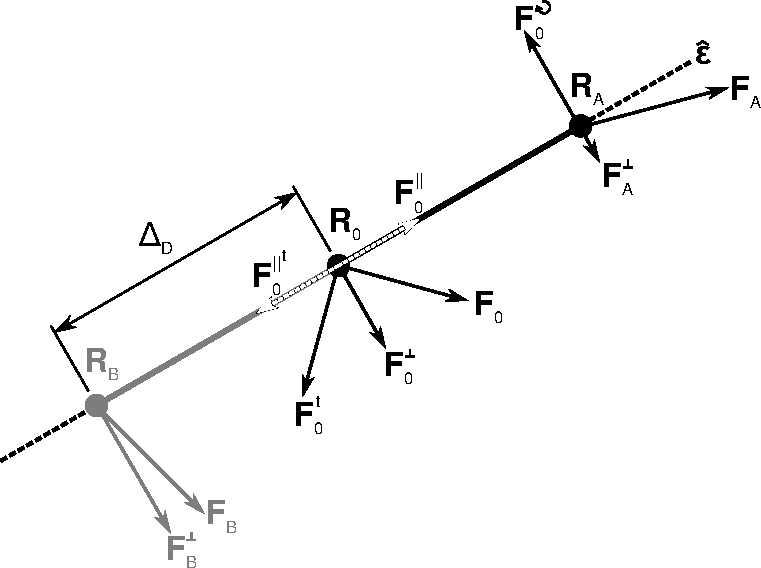
\includegraphics[width=0.6\linewidth]{dimer-force-overview}
\parbox{0.85\linewidth}{\caption{A schematic overview of the force components acting within the dimer method.
$\vR_\text{A}$ and $\vR_0$ are the positions of the dimer images with the greyed out $\vR_\text{B}$ as the virtual image (\fref{eq:dimer-point-extrapolate}).
Each force component is labeled with super- and subscripts as follow:
$0$, $\text{A}$ and $\text{B}$ in subscripts refer to at which point they are calculated,
$\perp$ and $\parallel$ in superscripts refer to the specific component of the full force (perpendicular and parallel to the minimum mode estimate, respectively),
$\text{t}$ in a superscript refers to the transformed force (\fref{eq:dimer-transform}),
$\circlearrowright$ refers to the rotational force (\fref{eq:rotational-force}) and no superscript refers to the gradient force.
$\Dsep$ is the distance between dimer points (\fref{eq:dimer-separation} and $\uvn$ is the current minimum mode estimate (or $\uvs$ during rotation).
}
\label{fig:dimer-force-overview}
}
  \end{center}
\end{figure}

\subsubsection{Gradient Transformation}
Once a minimum mode estimate is available for the current point, $\vR_0$, it is possible to transform the force so that any \sap1 is appears as a minimum.
As discussed in \fref{sec:saddle-points}, \sap{1}s are stationary (with zero gradient) and the Hessian has one and only one negative eigenvalue.
The goal is, thus, to maximize the function's value along the minimum mode while minimizing it along all other eigenmodes.
This can be achieved, simply, by inverting any force components along the minimum mode,
\beq{dimer-transform}
\vF_0^\text{t} = \vF_0 - 2(\vF_0 \cdot \uvn)\uvn.
\eeq
In cases were the dimer aligns itself with a contour of the potential in a convex region (where the Hessian has only positive eigenvalues), it is possible that a lot of time will be spent there.
In order to circumvent this, a different force transformation,
\beq{dimer-transform-minima}
\vF_0^\text{t} = -(\vF_0 \cdot \uvn)\uvn ,
\eeq
is often used in these regions.
This latter transformation simply inverts the force along the minimum mode while ignoring any other components.
This along with a fixed, artificially large, step size should yield less iterations spent near minima and more near \sap1s.~\cite{dimer-original-1999}

\subsubsection{Iterative Translation}
After the force has been transformed such that \sap1s appear as minima --- \sap1s, however, remain unchanged with regards to the function's value --- it is possible to use conventional algorithms for finding minima as long as they support a systematic increase in the function's value.
A finitie difference method was suggested in the original implementation~\cite{dimer-original-1999} while more recent papers~\cite{dimer-kastner-2008} have used other methods, such as the L-BFGS algorithm~\cite{lbfgs}.

\subsubsection{Usage in Atomic Simulations}
The Dimer method was developed within the context of atomic simulations, where the function in question is the PES and the variables the spatial degrees of freedom of each atom in the system.

Multiple scenarios can be envisioned where the Dimer method brightly shines, two of which will be briefly discussed.

\ben{dimer-usage}
\item Consider a method that is not able to fully converge to a \sap{1}, such as the Double Nudged Elastic Band, which yields a configuration close to the \sap{1} and a reasonably good estimate of the minimum mode.
In such a situation the Dimer will quickly, and at low computational cost, find the \sap{1} exactly.
~\cite{dneb-2004}
\item As discussed in \fref{sec:tst-timescale-problem}, performing long time-scale dynamics is difficult.
The dimer can be used to map all relevant \sap{1}s leading out of a basin\footnote{It is, of course, nearly impossible to find \emph{all} \sap{1}s associated with a basin and even more difficult to know when they have all been found and ref. \cite{dimer-sampling-2011} discusses efforts to that end.}, then using HTST (\fref{sec:htst}) to find the reaction rates for each \sap{1}, it is possible to construct a probability table of possible events.
Using this table of events within the Kinetic Monte Carlo formalism~\citemiss, it is possible to traverse the PES in an accelerated manner.
~\cite{akmc-2001}
\een

\subsubsection{Performance}
Since the Dimer heavily depends on finite difference methods, inaccurate gradients can, thus, render the method useless.
When used with classical potentials, this is not a problem, but when used with quantum mechanical forces, such as those provided by DFT, care must be taken to converge the electronic structure well.
